\chapter*{Introduction / Motivation (3 pgs)}
\addcontentsline{toc}{chapter}{Introduction}

	liquid helium discovery, 1908, Heike Onnes, liquid state at 4.2K, superfluid state below 2.17K, full phase diagram:

	\begin{figure}[h]
		\centering
		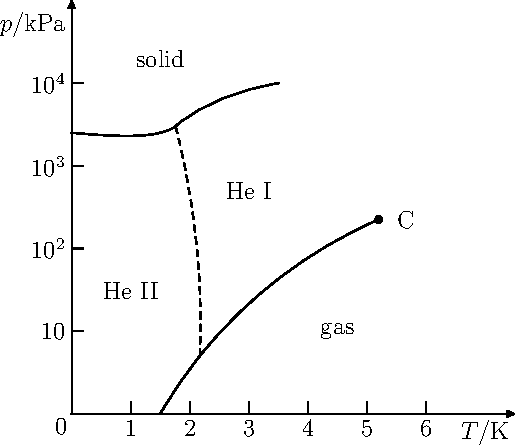
\includegraphics[width=0.5\textwidth]{graphics/theory/phase_diag}
		\caption{p-T diagram}
		\label{phase}
	\end{figure}

	labelling He-I, He-II, no solid state at 0K (weak van der Waals), only at 2.5MPa

	strange properties, thermal conductivity, negligible viscosity through capillaries

	Landau, Tisza: phenomenology, two-fluid model, proved bz rotating discs:

	\begin{figure}[h]
		\centering
		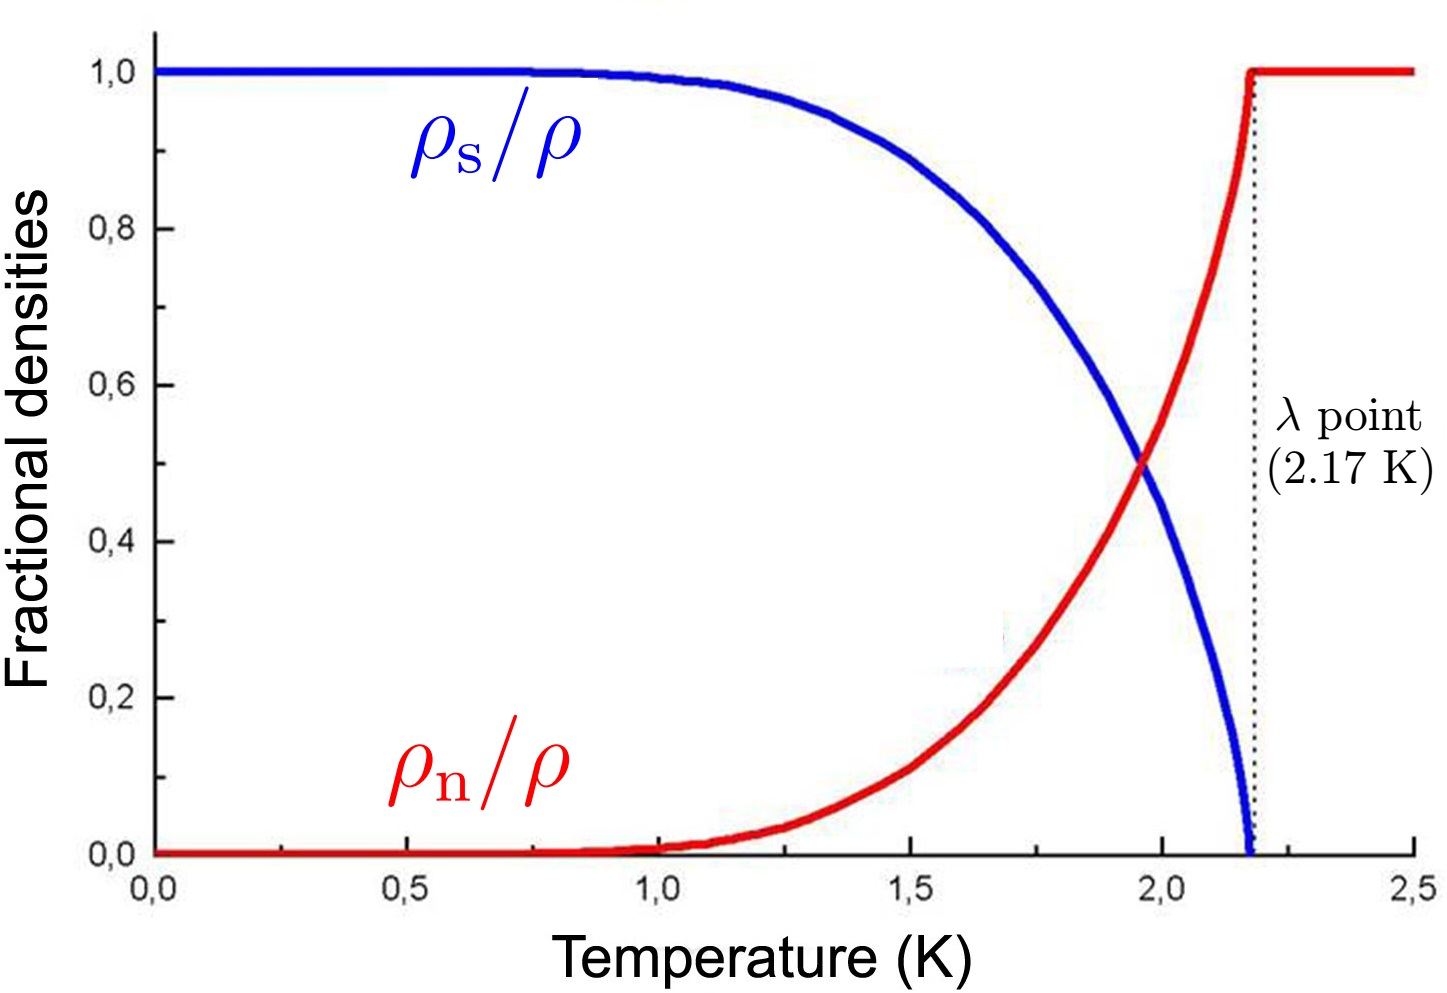
\includegraphics[width=0.5\textwidth]{graphics/theory/densities}
		\caption{temperature dependence of densities}
		\label{densities}
	\end{figure}

	London: similarity of superfluid component with orbiting electorns, macroscopic wave func

	irrotational fluid, quantum vortices, tangle:

	\begin{figure}[h]
		\centering
		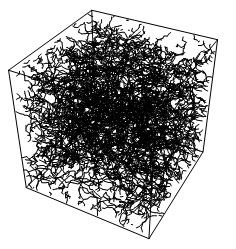
\includegraphics[width=0.5\textwidth]{graphics/theory/QT-tangle}
		\caption{Quantum Turbulence}
		\label{QT}
	\end{figure}

	CT experiments: transition to turbulence, drag coeffs

	QT experiments: coflow, counterflow, second sound

	QT vs CT: complicated N-S equations, critical velocity or Reynolds number, QT has probably more critical velocities

	Simulations: filament model, boundaries

	Motivations: investigate critical velocities and vortex density, create numeric model

	Goals: measure hydrodynamic profiles for more temperatures with oscillating object, transition from CT to QT, investifate numerically vortex rings

\newpage
\chapter{Theoretical Background (15 pgs)}

The theoretical part of this Thesis is composed of two chapters:

\begin{itemize}
	\item[1.] Mesoscopic view - theoretically cover London's theory, creation and numerical modelling of quantum vortex, vortex dynamics.

	\item[3.] Macroscopic view - hydrodynamics of two-fluid model, oscillatory motion in such fluid, creation of QT, existence and usage of second sound

\end{itemize}

Many of this is covered in textbooks and papers.

He properties, total spin, Bose gas, critical temperature, heat capacity

\newpage

{\Huge \bfseries Mesoscopic view}
\addcontentsline{toc}{chapter}{Mesoscopic model}
\vspace{0.3cm}

\section{London's theory}

Gross-Pitaevskii NLSE:

\begin{equation}
i \hbar \frac{\partial \psi}{\partial t} = - \frac{\hbar^2}{2m} \nabla^2 \psi - m\eps \psi + V_0 \vert \psi \vert^2 \psi
\end{equation}

Macroscopic wave function:

\begin{equation}
\psi(\vec{r},t) = \sqrt{\frac{\rho_{\ind s}}{m_4}}\, e^{i \phi (\vec{r},t)}\,,
\label{psi}
\end{equation}

London's idea, properties of $\psi$, zero vorticity

Circulation:

\begin{equation}
\Gamma = \oint_{\mathcal{C}} \vec{v_{\ind s}} \cdot \unit{d}\vec{\boldsymbol{\ell}}
\label{gamma}
\end{equation}

\begin{figure}[h]
	\centering
	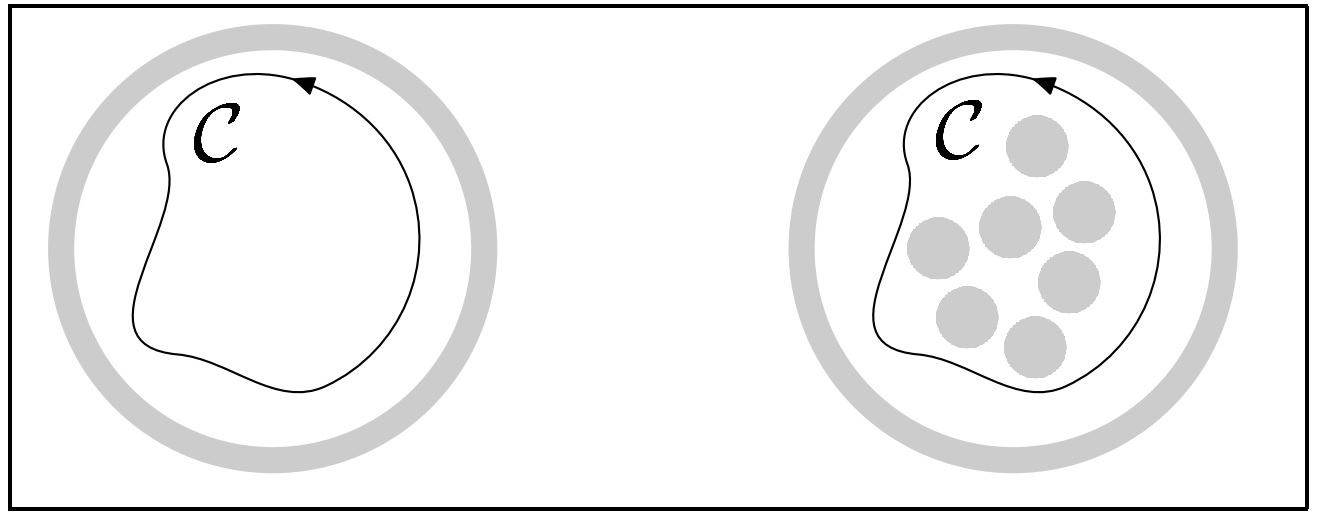
\includegraphics[width=0.5\textwidth]{graphics/theory/singularity}
	\caption{singularities within fluid}
	\label{singularity}
\end{figure}

\section{Quantum vortex}
\begin{itemize}
	\item definition
	\item induced velocity
	\item energy
	\item quantized circulation
	\item quantum turbulence
\end{itemize}

tiny vortex of size 1A, created with energetic excitation and $\psi$ collapse, core contains pure normal component, superfluid is circulating around, limitation by Landau critical velocity

Quantized circulation:

\begin{equation}
\Gamma = \frac{\hbar}{m_4} 2\pi n = \equiv n \kappa
\label{gamma}
\end{equation}

Ordering of vortices in rotating container:

\begin{figure}[h]
	\centering
	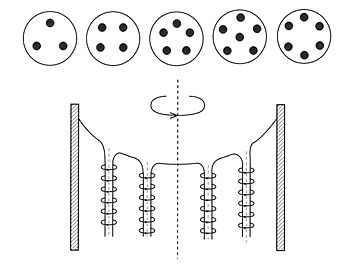
\includegraphics[width=0.5\textwidth]{graphics/theory/rotating-helium}
	\caption{Quantized vortices in rotating container}
	\label{rotating-helium}
\end{figure}

Superfluid velocity distirbution around vortex core:

\begin{figure}[h]
	\centering
	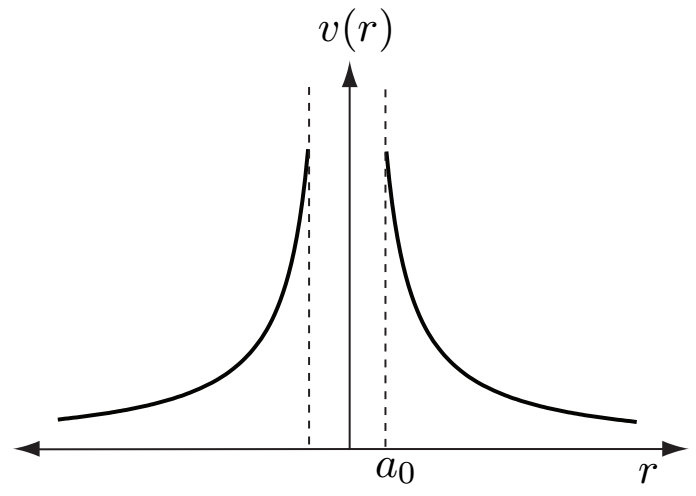
\includegraphics[width=0.5\textwidth]{graphics/theory/vortex_velocity}
	\caption{decrease of rotational velocity around vortex}
	\label{vortex_velocity}
\end{figure}


\section{Vortex filament model}
each segment know its position and neighbours, defining vectors $\vec{s}$, $\vec{s}^{\prime}$, $\vec{s}^{\prime\prime}$ + physical meaning, state definition

Associated vectors with segment:

\begin{figure}[h]
	\centering
	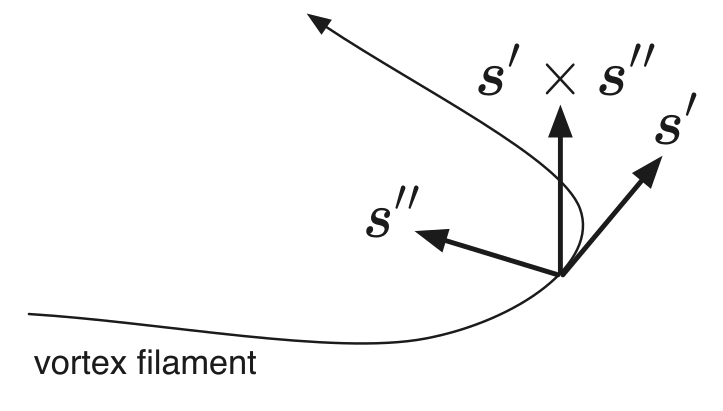
\includegraphics[width=0.5\textwidth]{graphics/theory/filament}
	\caption{vortex filament}
	\label{filament}
\end{figure}

Incompressibility:

\begin{equation}
\nabla \dot \vec{v}_s = 0
\end{equation}

Biot-Savart law:

\begin{equation}
\vec{v}_i(\vec{s}) = \frac{\Gamma}{4\pi} \int_{\mathcal{L}} \frac{(\vec{r} - \vec{s}) \times \text{d}\vec{r}}{\vert \vec{r} - \vec{s} \vert^3}
\end{equation}

Problems if $\vec{s}$ lies on the line

LIA approximation:

\begin{equation}
\vec{v}_i(\vec{s}) = \beta \vec{s}^{\prime} \times \vec{s}^{\prime \prime} + \frac{\Gamma}{4\pi} \int_{\mathcal{L}^{\prime}} \frac{(\vec{r} - \vec{s}) \times \text{d}\vec{r}}{\vert \vec{r} - \vec{s} \vert^3}
\end{equation}

LIA with substitued beta:

\begin{equation}
\vec{v}_i \approx \frac{\Gamma}{4\pi} \ln\Big(\frac{R}{a_0}\Big) \vec{\hat{b}}
\end{equation}

\begin{figure}[h]
	\centering
	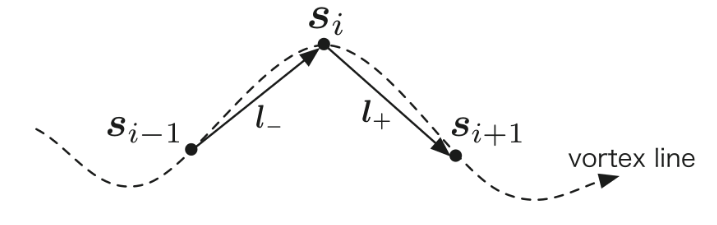
\includegraphics[width=0.5\textwidth]{graphics/theory/filament2}
	\caption{vortex filament 2}
	\label{filament2}
\end{figure}



\section{Vortex dynamics}
\begin{itemize}
	\item magnus force
	\item mutual friction
	\item Schwarz's equation
	\item special case - quantum ring (properties)
	\item Kelvis waves (?)
\end{itemize}

Magnus force:

\begin{equation}
\vec{f}_M = \rho_s \Gamma \vec{s}^{\prime} \times (\vec{v}_i - \vec{v}_{tot})
\end{equation}

Total velocty:

\begin{equation}
\vec{v}_{tot} = \vec{v}_s + \vec{v}_i
\end{equation}


Drive force (mutual friction):

\begin{equation}
\vec{f}_D = - \alpha\rho_s\Gamma\vec{s}^{\prime} \times [\vec{s}^{\prime} \times (\vec{v}_i - \vec{v}_{tot})] - \alpha^{\prime}\Gamma\vec{s}^{\prime} \times (\vec{v}_i - \vec{v}_{tot})
\end{equation}

Assuming no mass of vortex core:

\begin{equation}
\vec{f}_D + \vec{f}_M = 0
\end{equation}

Shwarz's equation:

\begin{equation}
\frac{\text{d}\vec{s}}{\text{d}t} = \vec{v}_s + \vec{v}_i + \alpha\vec{s}^{\prime} \times (\vec{v}_{ns} - \vec{v}_i) - \alpha^{\prime}\vec{s}^{\prime} \times [\vec{s}^{\prime} \times (\vec{v}_{ns} - \vec{v}_i)]
\end{equation}

Quantized vortex rings, its dynamics, velocity, life expectancy

Center motion:

\begin{equation}
v_{\text{center}} = \frac{\Gamma}{4\pi R} (\eta - 1/4)
\end{equation}

\begin{equation}
\eta = \ln(8R/a)
\end{equation}

Energy:

\begin{equation}
E = \frac{\rho \Gamma^2 R}{2} (\eta - 7/4)
\end{equation}


\begin{figure}[h]
	\centering
	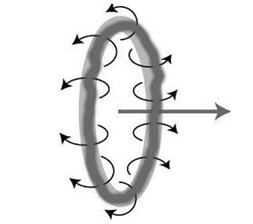
\includegraphics[width=0.5\textwidth]{graphics/theory/vortex-ring}
	\caption{dynamics of quantum vortex ring}
	\label{vortex-ring}
\end{figure}

Kelvin waves (?)

\newpage

{\Huge \bfseries Macroscopic view}
\addcontentsline{toc}{chapter}{Macroscopic model}
\vspace{0.3cm}

\section{Hydrodynamics of two-fluid}
\begin{itemize}
	\item Landau's assumptions
	\item two densities, velocities (+pic)
	\item updated hydrodynamical equations - HVBK
	\item dynamical similarity
	\item Reynolds number
\end{itemize}

HVBK equations:

\begin{align}
\frac{\partial\vec{v}_n}{\partial t} + (\vec{v}_n\cdot \nabla)\vec{v}_n =& -\frac{1}{\rho} \nabla P - \frac{\rho_s}{\rho_n} S \nabla T + \nu_n \nabla^2 \vec{v}_n + \vec{F}_{ns}\,,
\label{motion_normal}\\
\frac{\partial\vec{v}_s}{\partial t} + (\vec{v}_s\cdot \nabla)\vec{v}_s =& -\frac{1}{\rho} \nabla P + S \nabla T + \vec{T} - \frac{\rho_n}{\rho} \vec{F}_{ns}\,,
\hspace{15mm}
\label{motion_super}
\end{align}

, where we have defined:

\begin{equation}
\vec{\Omega}_s = \nabla \times \vec{v}_s\,,
\end{equation}
\begin{equation}
\vec{F} = \frac{B}{2} \vec{\hat{\Omega}} \times [\vec{\hat{\Omega}}_s \times (\vec{v}_n - \vec{v}_s - \nu_s\nabla \times \vec{\hat{\Omega}})]
+ \frac{B^{\prime}}{2} \vec{\Omega}_s \times (\vec{v}_n - \vec{v}_s - \nu_s\nabla \times \vec{\hat{\Omega}}_s)\,,
\end{equation}
\begin{equation}
\vec{\hat{\Omega}}_s = \vec{\Omega}_s / \vert \vec{\Omega}_s \vert\,,
\end{equation}
\begin{equation}
\vec{T} = -\nu_s \vec{\Omega}_s \times (\nabla \times \vec{\hat{\Omega}}_s)
\end{equation}
\begin{equation}
\nu_s = \frac{\Gamma}{4\pi} \log(b_0 / a_0)
\end{equation}

\begin{figure}[h]
	\centering
	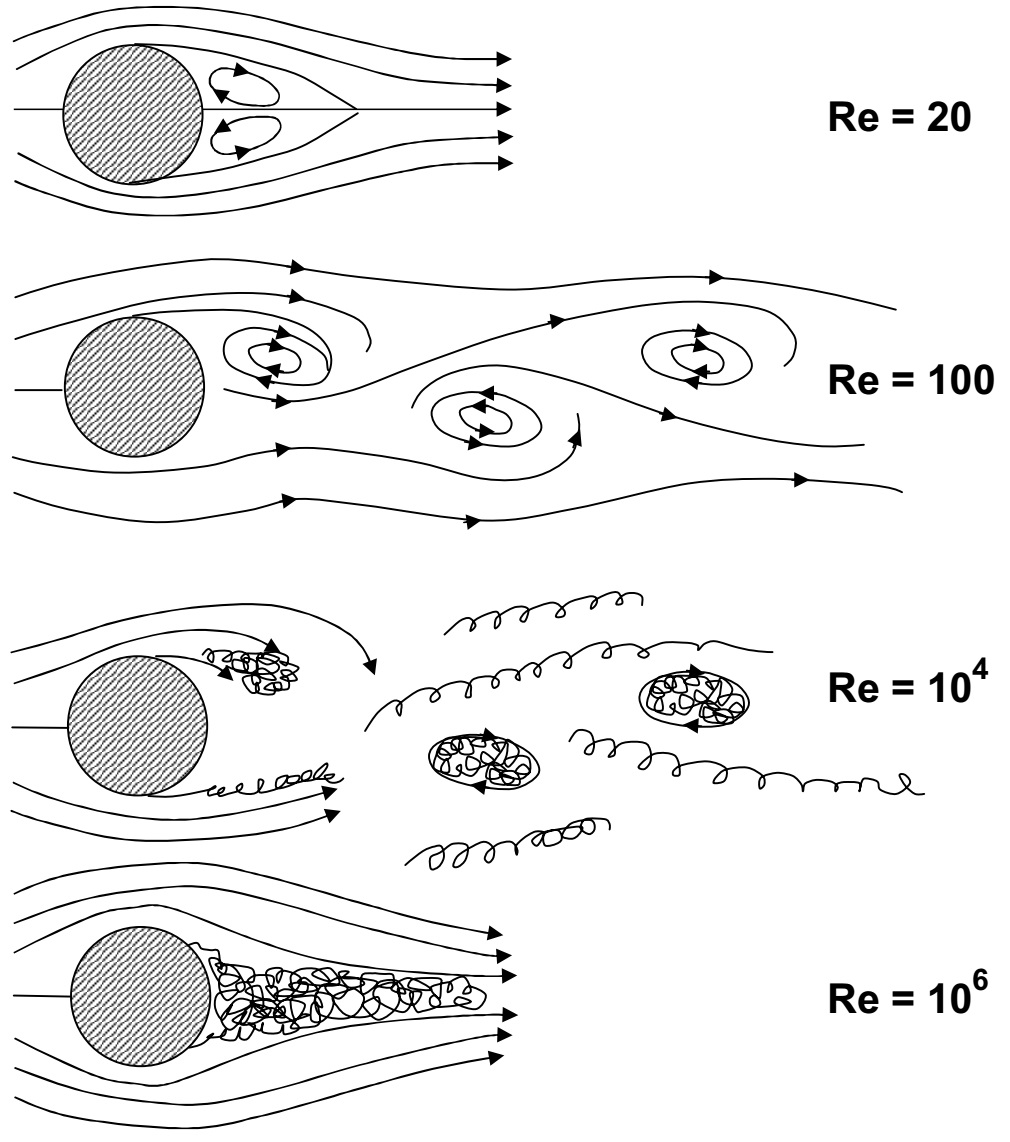
\includegraphics[width=0.5\textwidth]{graphics/theory/laminar-turbulent}
	\caption{transition from laminar to turbulent flow}
	\label{laminar-turbulent}
\end{figure}

\begin{figure}[h]
	\centering
	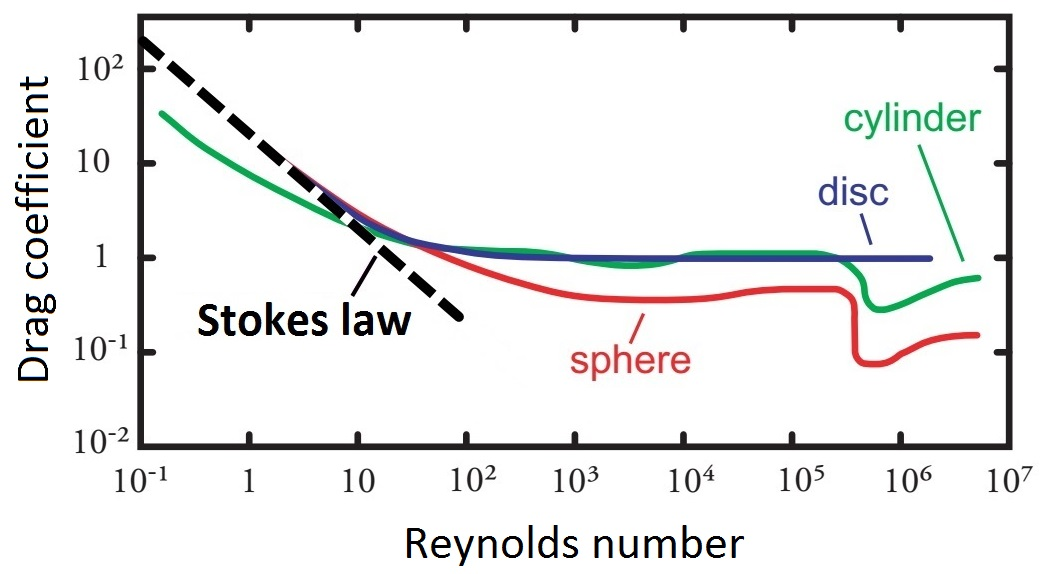
\includegraphics[width=0.5\textwidth]{graphics/theory/C-Re}
	\caption{drag coeffs of different objects}
	\label{C-Re}
\end{figure}

Drag coeff:

$$
C_D \!\propto\! v^\alpha, \hspace{1cm}
\text{where}
\left\{
  \begin{array}{l l}
    \alpha=-1 & \quad \text{for $\Re \in (0-10)$}\\
    \alpha=0 & \quad \text{for $\Re \in (10^3-10^5)$}
  \end{array}
\right.\,.
$$


\section{Oscillatory motion in superfluid}
\begin{itemize}
	\item penetration depth
	\item Re for oscillations
	\item defining depth and Re separately for normal and superfluid components
\end{itemize}

Attenuated wave:

\begin{equation}
\vec{v} \propto e^{-\vert\vec{r}\vert/\delta} \vec{\hat{e}}_{\vec{r}}(\omega, t)\,,
\label{v_pen}
\end{equation}

Penetration depth:

\begin{equation}
\delta = \sqrt{\frac{2\nu}{\omega}}\,.
\label{penetration}
\end{equation}

Oscillatory Reynolds number:

\begin{equation}
\Re_{\delta} = \frac{v_0 \delta}{\nu} = \frac{v_0}{\sqrt{\nu \pi f}} \,.
\label{Re*}
\end{equation}

Depth and $\Re$ for normal component:

\begin{equation}
\delta_{\ind n} = \sqrt{\frac{2\eta}{\rho_{\ind n}\omega}}\,,
\hspace{1cm}
\Re_{\ind n} = \frac{v_0 \delta_{\ind n} \rho_{\ind n}}{\eta}
\label{twofluid}\,.
\end{equation}


\section{Quantum turbulence}
\begin{itemize}
	\item critical velocity according to landau
	\item critical velocity scaling in oscillatory case
	\item T dependence of critical velocities (Bc. results)
\end{itemize}

Critical velocity scaling:

\begin{equation}
v_{\text{crit}} \propto \sqrt{\omega}
\end{equation}

\begin{figure}[h]
	\centering
	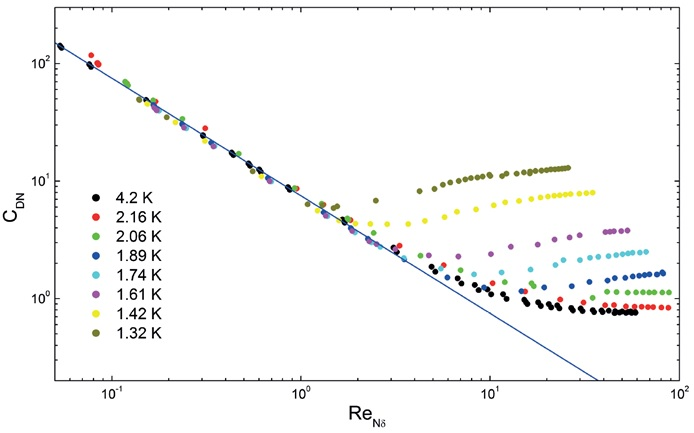
\includegraphics[width=0.5\textwidth]{graphics/theory/C-Re_normal}
	\caption{drag coeffs vs Reynolds number of normal component}
	\label{C-Re_normal}
\end{figure}

\section{Second sound}
\begin{itemize}
	\item what it is
	\item velocity of second sound
	\item attenuation
	\item vortex line density estimate
\end{itemize}

\begin{equation}
\vec{v}_{\ind{ns}} \propto e^{-\alpha z} \vec{\hat{e}}_{\vec{r}}(\vec{k},\vec{r},\omega,t)\,,
\end{equation}

\begin{equation}
\alpha = \frac{B\kappa L}{6 c_2}
\label{alpha_mean}\,.
\end{equation}


First and second sounds:

\begin{figure}[h]
	\centering
	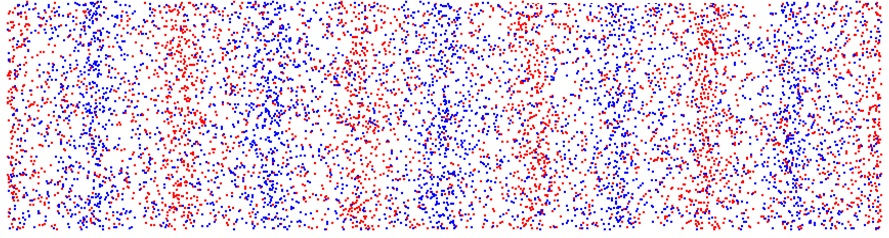
\includegraphics[width=0.7\textwidth]{graphics/theory/ss_1}
	\caption{first mode of second sound}
	\label{ss_1}
\end{figure}

\begin{figure}[h]
	\centering
	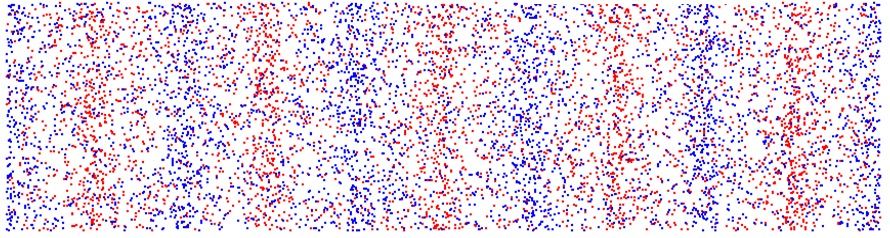
\includegraphics[width=0.7\textwidth]{graphics/theory/ss_2}
	\caption{second mode of second sound}
	\label{ss_2}
\end{figure}

Velocity of second sound with temperature:

\begin{figure}[h]
	\centering
	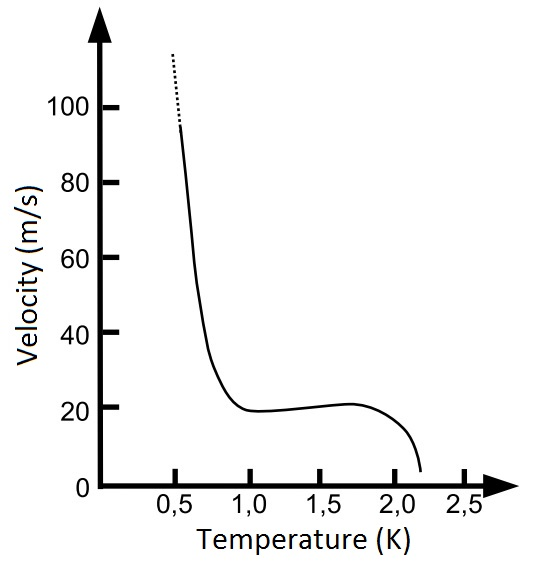
\includegraphics[width=0.3\textwidth]{graphics/theory/ss_velocity}
	\caption{velocity of ss with temperature}
	\label{ss_velocity}
\end{figure}

Vortex line density:

\begin{equation}
L = \frac{6\pi \Delta f_0}{B\kappa}\bigg( \frac{A_0}{A} - 1 \bigg)\,,
\label{L}
\end{equation}


\newpage
